\section{Vision}
Computer vision is used to detect and locate objects that the robot can collect. QR codes are used to store information about each object, such as its form, color, and size. This information can be stored in a database so the object can be found in the storage system and returned to the user.

\texttt{OpenCV} was chosen because it is a widely used and well-documented library for working with computer vision. It simplifies the development of computer vision applications by providing established implementations of many fundamental image-processing functions, reducing the need to implement these methods from scratch. \texttt{OpenCV} already has functions to find, read, and generate QR codes, along with functions to estimate an object's position and rotation relative to the camera.
\texttt{OpenCV} also handles camera-related tasks, such as taking images, setting the resolution, and adjusting other camera settings. This removes the need for a separate tool to control the camera and provides the functions needed to calibrate it.

\subsection{Getting the Object's Location}
To pick up an object, its location relative to the robot arm must be determined. This process can be split into smaller parts, such as finding the object and calculating its position from the camera perspective.

When trying to find an object in a picture, people look for features that make the object easy to identify. This is often something like the outline of the object. However, if only the edge of an object is used, the detected point can be placed anywhere along that edge. A corner is therefore more useful, because if it is moved slightly, it is easier to see that it is no longer correctly placed \cite{opencv_features}.
For the computer to find the object, simple features must therefore be present in the image. For this project, QR codes were chosen.



\subsection{QR Codes}

\begin{wrapfigure}[5]{r}{0.20\textwidth}
    \vspace{-80pt}
    \centering
    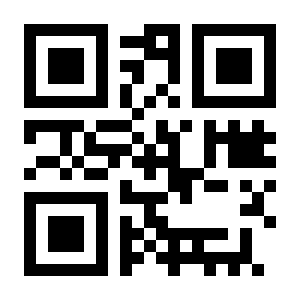
\includegraphics[width=0.18\textwidth]{figures/qr_code_raw_red.png}
    \captionsetup{font=small}
    \caption{Example of a simple QR code used to locate and store information about the objects}
    \label{fig:QR-Code-side}
\end{wrapfigure}

QR codes are used both as features for the computer to detect and as a way to store information about the object. These features stand out in the construction of a QR code; see \cref{fig:QR-Code-side} for an example. Three of the corners contain large squares, which are the features the computer can look for. These are also what the \texttt{QRCodeDetector} looks for when finding QR codes.



\begin{wrapfigure}[7]{r}{0.20\textwidth}
    \vspace{-30pt}
    \centering
    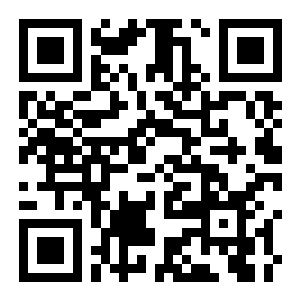
\includegraphics[width=0.18\textwidth]{figures/qr_code_Json_red.png}
    \captionsetup{font=small}
    \caption{Example of a detailed QR code where the information is more difficult for computer vision to read}
    \label{fig:QR-Json}
\end{wrapfigure}

When looking for QR codes, the amount of detail can make them harder to find and read. Since the QR code must fit on the objects that will be picked up, a more detailed QR code means that the individual pixels become smaller. As shown in \cref{fig:QR-Code-side} and \cref{fig:QR-Json}, this can make them harder for the computer to detect.

\subsubsection{Test}
To find out whether the detailed QR code or the simpler QR code worked better, we tested how often each QR code was found and read successfully. This was tested at different heights to see how consistent the detection was and to find a suitable camera height. All tests at different heights and with different QR codes were performed using 1000 images.


\begin{table}[H]
\centering
\begin{tabular}{|c|c|c|}
\hline
Distance from camera to table & detailed & Simple \\
\hline
50 cm & 57,9\% & 96,0\% \\
\hline
55 cm & 75,2\% & 99,5\% \\
\hline
60 cm & 36,5\% & 98,6\% \\
\hline
65 cm & 15,4\% & 81,8\% \\
\hline
70 cm & 62,2\% & 53,4\% \\

\hline
\end{tabular}
\caption{Visions ability to read QR codes at different distances}
\label{tab:vision-readability}
\end{table}

From the data in \cref{tab:vision-readability}, it is clear that the vision setup is much more consistent at reading the simpler QR code. The results showing how consistently the setup found the QR codes can be seen in \cref{tab:appendix-vision-findability} in Appendix~\ref{app:Vision-test}. In general, the setup was very consistent at finding the QR codes at the different distances. When choosing the best camera distance, the goal was to use the highest point where detection was still consistent, giving the robot arm as much free space to move as possible. The reading results show a sharp drop-off at \texttt{60 cm}. Therefore, the simpler QR code and a camera height of \texttt{60 cm} were chosen for this project.



\subsection{Perspective-n-Point (PnP)}
After the object has been found in the image, the QR code can be used to calculate its position. Because all the QR codes are the same size, their known dimensions make it possible to calculate the object's location relative to the camera, which can then be converted into coordinates for the robot arm to move to.

For the \texttt{PnPsolve} function from \texttt{OpenCV} to calculate an accurate position, the function must be calibrated to the camera. All cameras distort or warp the images in some way, so the camera distortion must be determined. This calibration only has to be done once for the camera when the height is set. 
The calibration was made with a Charuco board; see Appendix~\ref{app:charuco-board}.



